%!TEX root = ../SciVis.tex
Besides the height plot we also implemented stream tubes, which are also drawn in three-dimensions. Stream tubes trace particles through a vector field as cylindrical tube. In contrast, to  height plots, stream tubes visualize a three-dimensional dataset. 

Therefore we need to construct a 3D dataset out of our 2D dataset by using time as the third axis. Basically, we store the last $n$ timeslices of our 2D dataset to create a data cube. 

We designed this data cube as a circular buffer. We decided to store all data that becomes available in every simulation step (i.e. rho,vx,vy,fx,fy). This gives us a greater flexibility since we are able to calculate all kinds of conversion on the fly (e.g. $|v|$).  
Deque and vector have been used to define the circular buffer as \verb| deque<vector<vector<fftw_floats> > > >|.  A deque  allows to easily push and pop data at both ends, which makes the implementation easier. 
We used the available STL data structures because they are reliable and effiecent.
The RHO value of a sample point $sp$  at timestep $t$ can be accessed via  \verb|buffer[t][RHO][sp]|. The data structure has been wrapped in a class to allow uniform access and provide general purpose methods. 


If we visualize this dataset by using a simple hedgehog glyph technique as described previously 
 \begin{figure}[htbp]
 \centering
 \begin{minipage}[t]{0.48\textwidth}
 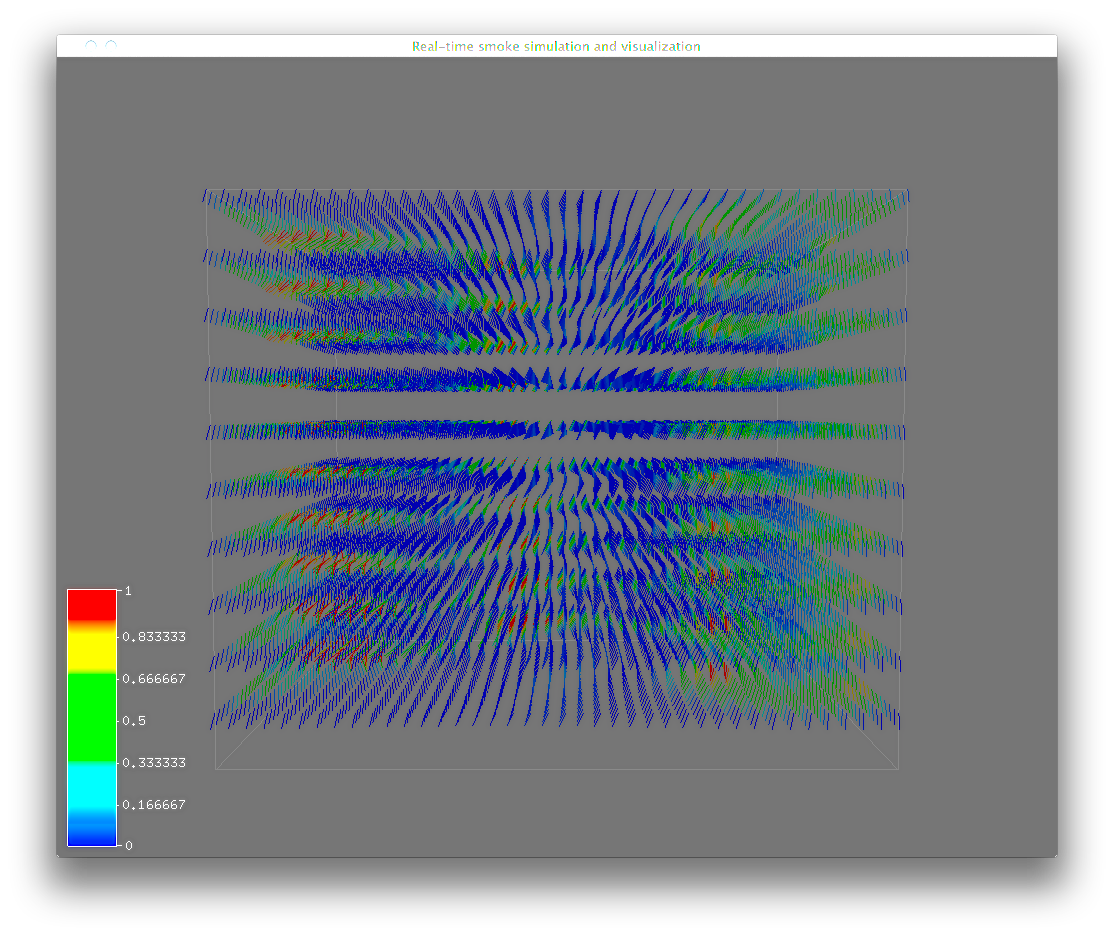
\includegraphics[height=3in]{figures/streamtubes/30datacube_bottom.png}
 \caption{Hedgehog visualization of the time-dependent velocity vector field. The individual time-slices are clearly visible if viewed from below.}
 \label{fig:datacube_bottom}
 \end{minipage}\hspace{.04\textwidth}%
 \begin{minipage}[t]{0.48\textwidth}
 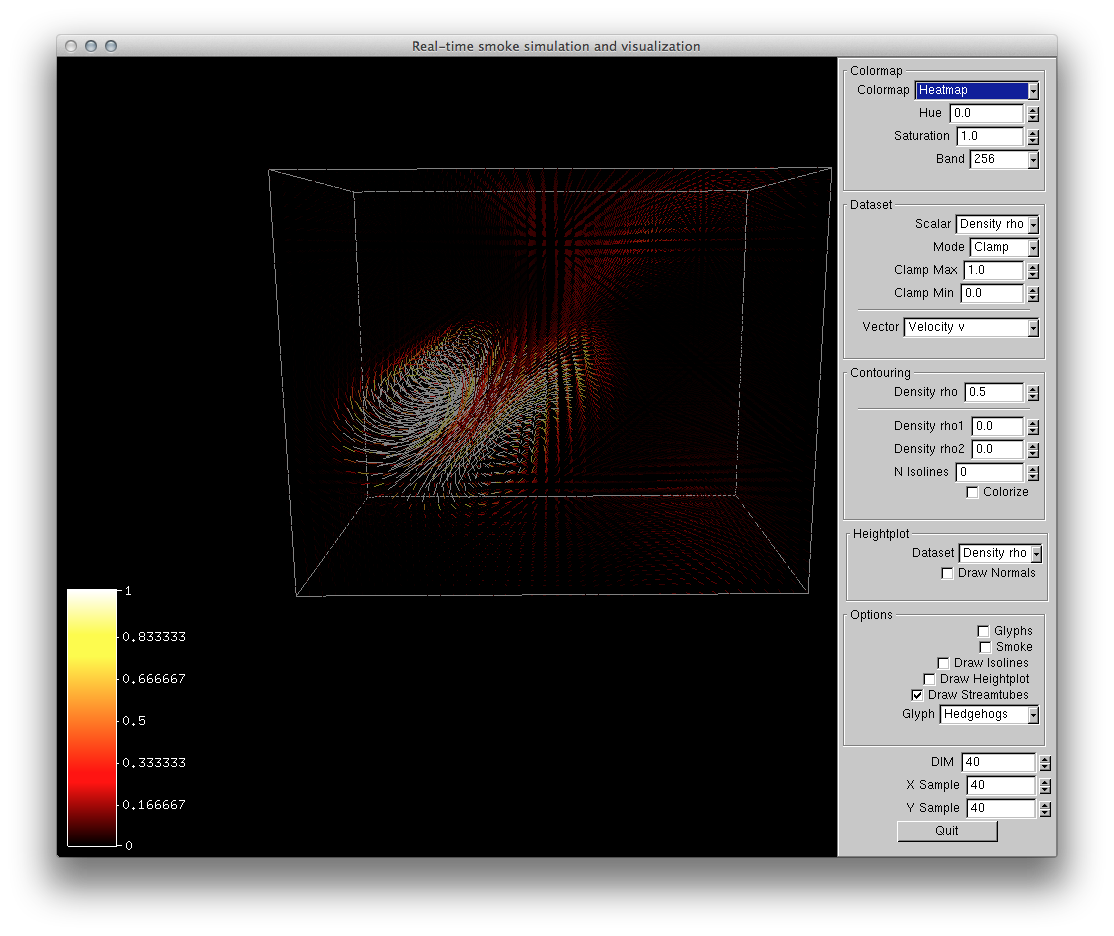
\includegraphics[height=3in]{figures/streamtubes/31datacube_front.png}
 \caption{Frontal view of the the time-dependent velocity vector field. Occlusion is a problem as the individual vectors/timeslices cannot be easily perceived.}
 \label{fig:}
 \end{minipage}
 \end{figure}
 
 
 place (and remove) seed points in the 3D volume.
 control the (x,y,z) position of a seed point by means of sliders. 
 allow users to click in some point in the window. 
 
 
 accomodate three dimensions instead of two.
 
 triliniear interpolation
    
    
pushed on 2D-vector that contains the actual pixel values of the streampoints + the scalar value at that point




  
  construct a stream tube geometry around it. 
  asubsequent step is to use a circle sampled as a closed polyline with n points, user-controlled

   For each sample point pi along a streamline, construct such a cross-section. The cross-section should be orthogonal to the current polyline segment pi, pi+1.

  
\begin{lstlisting}[language=C,caption={Cross-section in 3D reference frame}]
glBegin(GL_QUAD_STRIP);
  for (int i = 0; i <= 360; i = i + (360 / n)) {
    float theta = i * (M_PI / 180);
    float theta2 = (i + 1)*(M_PI / 180);
    
    float normal[3] = {};
    float vz[3] = {
        (cos(theta) * r) - (cos(theta) * rn),
        (sin(theta) * r)-(sin(theta) * rn),
         10 
    };
    float vx[3] = {
        (cos(theta) * r) - (cos(theta2) * r),
        (sin(theta) * r)-(sin(theta2) * r),
        0
    };
    normalize3(vz);
    normalize3(vx);
    crossproduct(vz, vx, normal);

    setColor(points[sp][3], TEXTURE);
    glNormal3f(normal[0], normal[1], normal[2]);
    glVertex3f(cos(theta) * r, sin(theta) * r, 0);

    setColor(points[sp + 1][3], TEXTURE);
    glNormal3f(normal[0], normal[1], normal[2]);
    glVertex3f(cos(theta) * rn, sin(theta) * rn, 15);

    setColor(points[sp][3], TEXTURE);
    glNormal3f(normal[0], normal[1], normal[2]);
    glVertex3f(cos(theta2) * r, sin(theta2) * r, 0);

    setColor(points[sp + 1][3], TEXTURE);
    glNormal3f(normal[0], normal[1], normal[2]);
    glVertex3f(cos(theta2) * rn, sin(theta2) * rn, 15);
  }
glEnd();
\end{lstlisting}  
  
 
 
 how to exactly place the cross-section? 
 
 a full reference frame in 3D, placed at each streamline point, which indicates the exact position and orientation of the cross-section. 
 
 get direction, local and up vector
 rotation matrix
 gets 'swept' along it


 \begin{lstlisting}[language=C, caption={Rotation and translation matrix to move cross-section along the streamtube.}]
 GLfloat R[16] = {
     local[0]     , local[1]     , local[2]     , 0,
     up[0]        , up[1]        , up[2]        , 0,
     target[0]    , target[1]    , target[2]    , 0,
     points[sp][0], points[sp][1], points[sp][2], 1
 };
 glMultMatrixf(R);
 \end{lstlisting}
 
 shading and coloring of the stream tubes: use either flat or Gouraud shading, and either a constant color,
 
 just use the colormapping functionalities from step 2. 
 the scalar field can be selected in the user interface
 a color map which shows one of the scalar fields along the streamline, such as velocity vector magnitude |v| or density rho.


(diameter) of the streamtubes. 
linearly scaled to show one of the scalar field values in the simulation, such as velocity vector magnitude |v| or density rho. 
all fields
affected by the radius of the next seed points



\begin{figure}[htbp]
\centering
\begin{minipage}[t]{0.48\textwidth}
        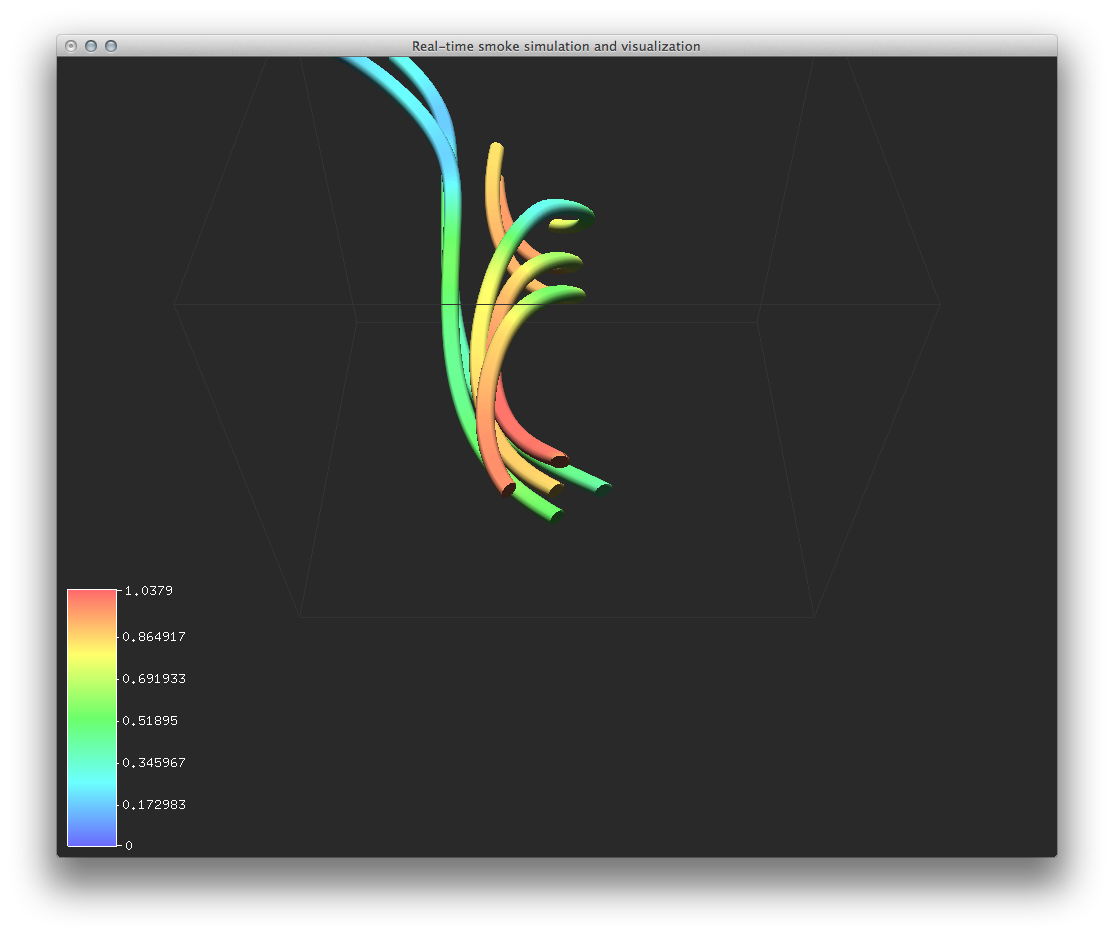
\includegraphics[height=3in]{figures/streamtubes/10tubes.png}
\caption{Combination of streamtubes and colormapping. Both techniques show the velocity. The seedpoints are centered in middle of the dataset.}
\label{fig:}
\end{minipage}\hspace{.04\textwidth}%
\begin{minipage}[t]{0.48\textwidth}
    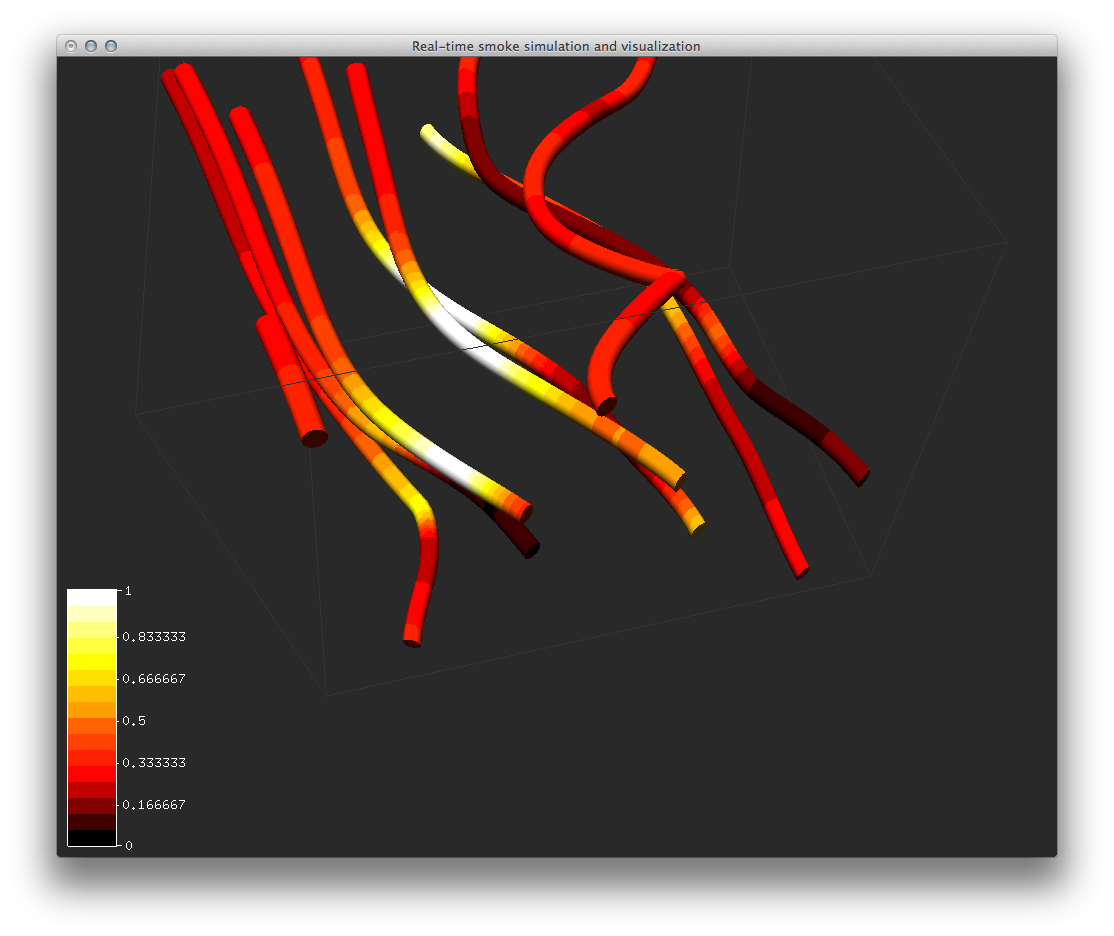
\includegraphics[height=3in]{figures/streamtubes/21banding_velodensity.png}
    \caption{Visualization of the velocity as streamtubes and density as heat colormap with a reduced number of colors. The banding effect makes the integration steps visible.}
    \label{fig:}
\end{minipage}
\end{figure}    

\begin{figure}[htbp]
\centering
\begin{minipage}[t]{0.48\textwidth}
        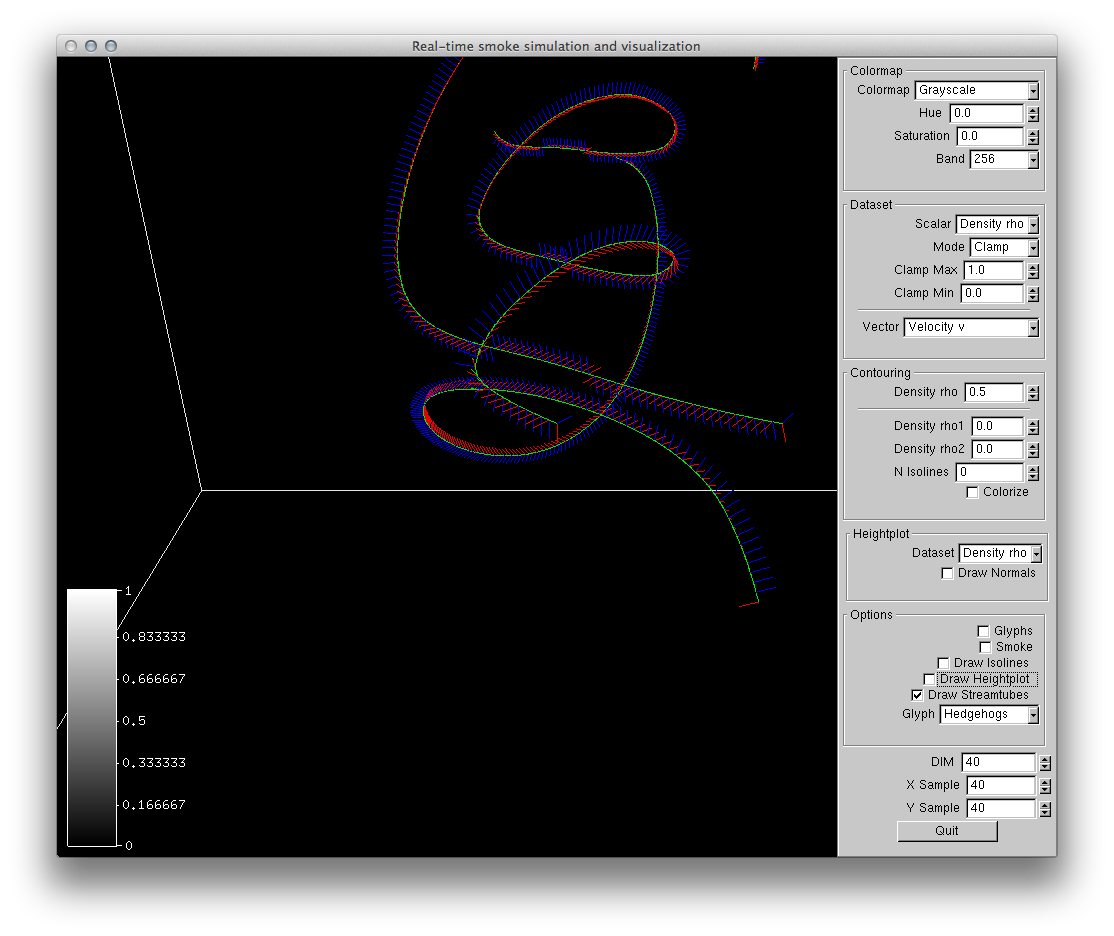
\includegraphics[height=3in]{figures/streamtubes/uvp.png}
\caption{Scaled orientation vectors. The green vector is tangent to the streamline, while the red and blue are perpendicular to the streamline.}
\label{fig:}
\end{minipage}\hspace{.04\textwidth}%
\begin{minipage}[t]{0.48\textwidth}
               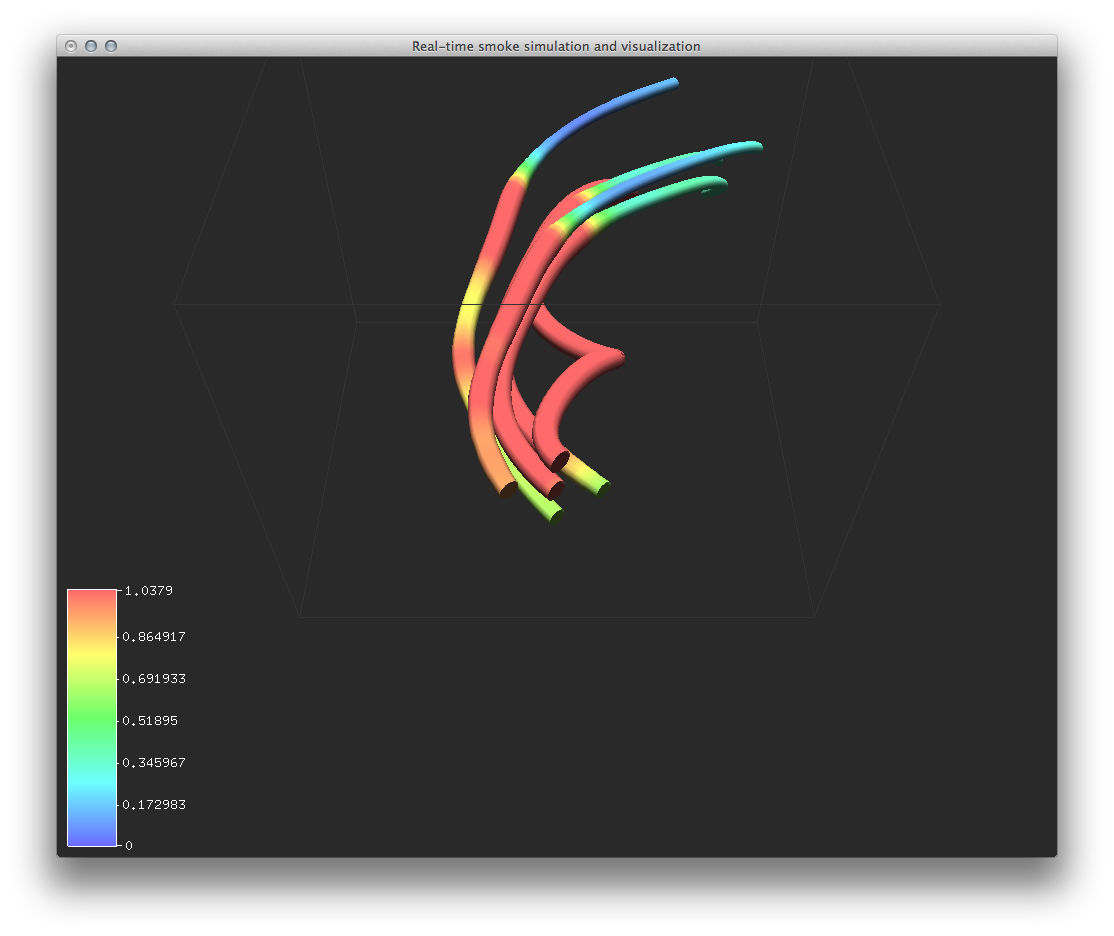
\includegraphics[height=3in]{figures/streamtubes/11thickTubes.png} 
    \caption{The diameter of the tube is linearly scaled based on a scalar value.}
    \label{fig:}
\end{minipage}
\end{figure}



\begin{figure}[htbp]
\centering
\begin{minipage}[t]{0.48\textwidth}
        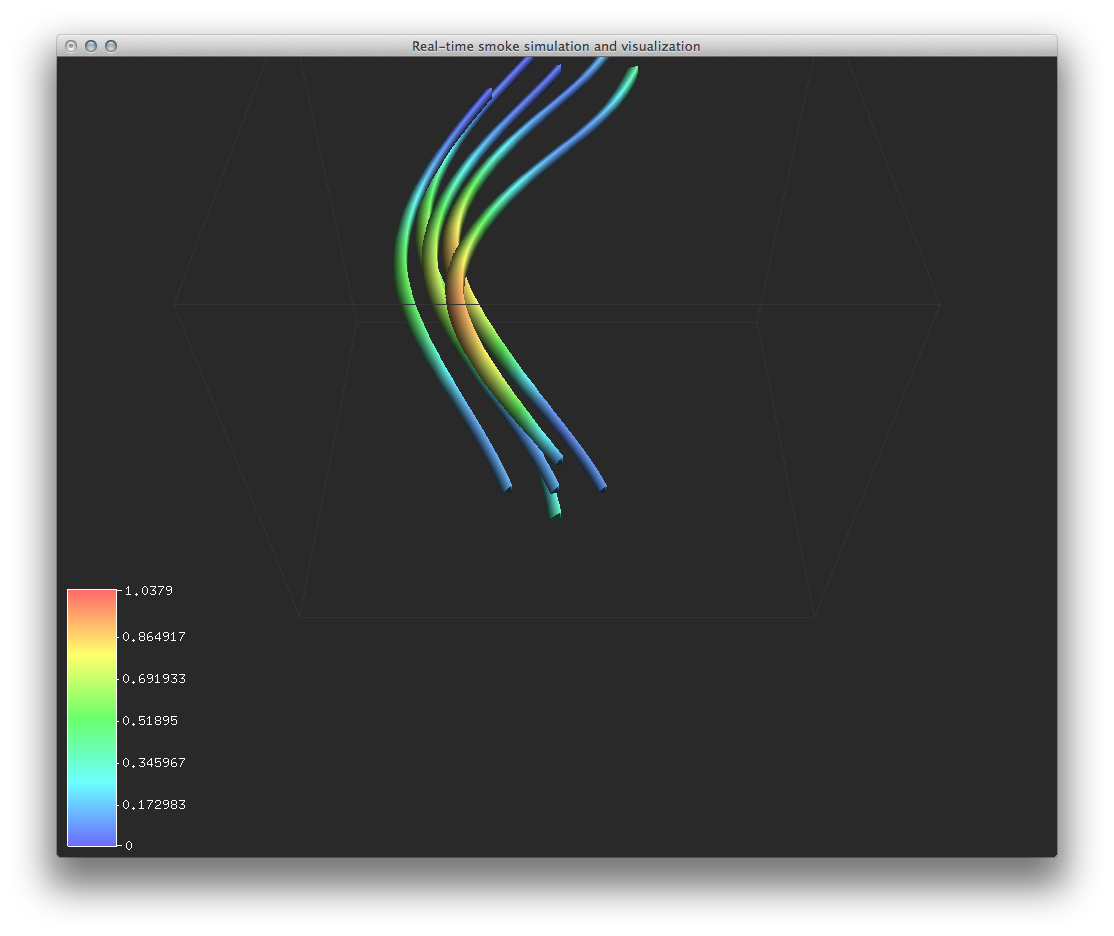
\includegraphics[height=3in]{figures/streamtubes/40threeSegments.png}
\caption{Triangular Tube geometry. The number of segments of the cross-sections can be adjusted dynamically.}
\label{fig:}
\end{minipage}\hspace{.04\textwidth}%
\begin{minipage}[t]{0.48\textwidth}
        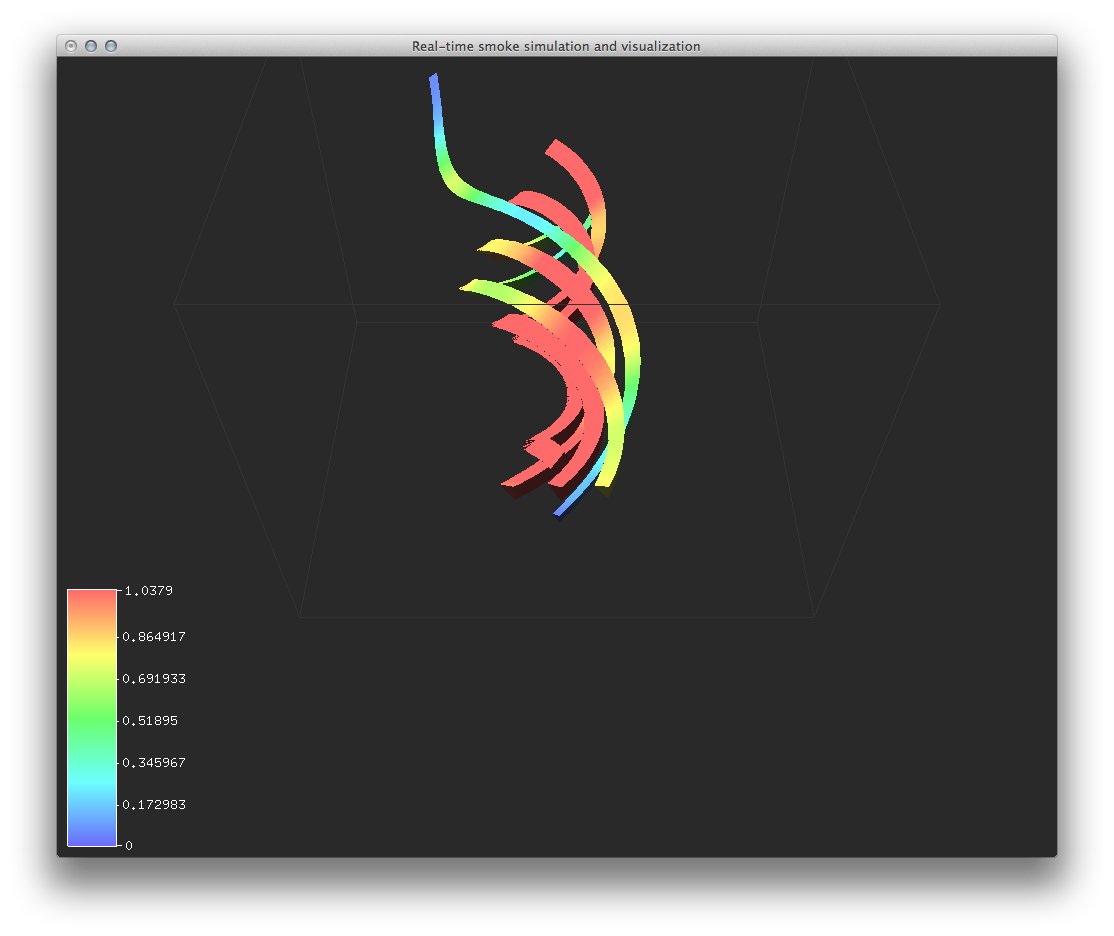
\includegraphics[height=3in]{figures/streamtubes/41flatshading.png}
    \caption{Flat shading accentuate the sharp-edges of the cross-section}
    \label{fig:}
\end{minipage}
\end{figure}

